\documentclass{article}
\usepackage{graphicx}
\usepackage{wrapfig}
\usepackage{lipsum}
\usepackage[skip=8pt,font=scriptsize]{caption}
\usepackage{subfig}
\usepackage{float}
\usepackage{fancyhdr}
\usepackage[letterpaper, portrait, margin=1.5in]{geometry}

\setlength{\parindent}{4em}
\setlength{\parskip}{0em}
\renewcommand{\baselinestretch}{1.15}
 
\pagestyle{fancy}
\fancyhf{}
\rhead{}
\lhead{}
\rfoot{Hasse Page \thepage}
\renewcommand{\headrulewidth}{0pt}

 
\begin{document}

\noindent 
Measurement of the Quenching Factor for Barium Fluoride Crystals\\
Ariel Hasse\\
Professor David Hitlin\\
California Institute of Technology\\


\section{Abstract}
The energy of particles can be determined by measuring the scintillation light emitted by crystals such as barium fluoride. As the particles travel through the inorganic scintillator, Birk’s Law describes the amount of light emitted for a given energy lost. The ratio of dispersed energy is dependent on the mass of the particle; this is known as the quenching factor. Barium fluoride has two mechanisms of scintillation, a fast and a slow component, which are at different wavelengths, that determine how quickly photons are emitted. The ratios of energy from the fast and slow components from multiple photomultiplier tubes with varying quantum efficiency as a function of wavelength, determine the final quenching factor. We find that the quenching factors of the fast and slow components are substantially different.
We measure the response of the barium fluoride crystal fast and slow components to alpha particles of known energies coming from the decay of slight radium contamination in the crystals. Confirmation with the known values allows for analysis of energy readout from gamma, electron, and alpha particles. This data, along with the quenching factor, is valuable for many high-energy physics experiments in which inorganic scintillators are used to find the mass or energy of particles. We will also use the findings to study the physical mechanisms affecting the quenching factor.


\section{Introduction}

In high energy physics the energy of a particle can be determined using a calorimeter in an accelerator. Calorimeters are composed of scintillators which are materials or compounds that emit light following particle interactions. Barium Flouride ($BaF_2$) crystals are inorganic scintillators that can be used for calorimeters. $BaF_2$ is of particular interest because it has two mechanisms of scintillation, a fast and a slow component. These are the two decay mechanisms that describe how quickly light is emitted through the lattice. For $BaF_2$ crystals the fast component is .6 ns and the slow component is 540 ns. Generally inorganic scintillators responses are slower than organic scintillators, however $BaF_2$'s fast component emits light very quickly. A short decay mechanism provides a clearer resolution and allows for more successive events to be detected. In order to benefit from the short decay time the scintillation light from the fast component must be seperated from the slow component. The relationship can be described by the non-linear energy loss through the lattice, known as Birk's constant or the quenching factor. Birk's Law describes how energy is lost as a particle flows through a scintillator. The proportion of energy lost is experimentally dependent on the mass of the interacting particle. The quenching factor is linearly dependent on energy and is different for the fast and slow component. The relationship is in the form of $\alpha_Q = E_f * \alpha_f + E_s * \alpha_s$ where $\alpha_Q$ is the quenching factor for a given light detector and energy level, $E_f$ and $E_s$ are the proportions of fast and slow scintillation, respectively, where $E_f + E_s = 1$, and $\alpha_f$ and $\alpha_s$ are the quenching factors for the fast and slow component at a given energy. In our research we determine the quenching factor for alpha particles as a function of energy for the fast and slow components of Barium Fluoride.

As photons exit the crystal they are recorded by a light sensor that reports the energy of the photon from its wavelength. Sensors have varying quantum efficiencies that allow different wavelengths to be detected and therefore different ratios of the fast and slow component. For each PMT the expected output, calibration term, from a particle can be determined using low mass decays such as gamma or electron sources with known keV values. Then we measure the scintillation from alpha particles, which by nature of their mass is affected by non-linear energy loss.The quotient of the expected energy and the observed energy, after converting with the calibration factor, describes the quenching factor, $\alpha_Q$, at the given energy for that PMT. 

The proportion of energy from the fast and slow component is then determined from the convolution of the emission spectrum of $BaF_2$ [Figure 1] and the quantum efficiency of the PMT. The convolution gives the relative light intensity per wavelength of light. The data is best represented by four gaussian functions where the first two correspond to the fast component and the last two correspond to the slow component. The integral of the curve is the total energy. The area under the first two gaussians is the percentage of energy from the fast component, $E_f$ and the area under the second two gaussians is the percentage of energy from the slow component, $E_s$. 

\begin{figure}
  \centering
    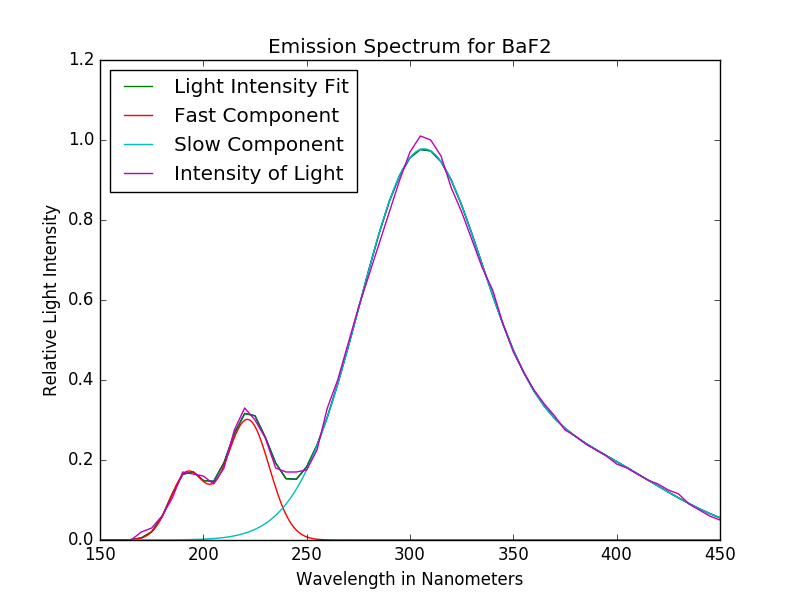
\includegraphics[width=0.5\textwidth]{FitsBaF2.png}
  \caption{Fitted Emission Spectrum for $BaF_2$ crystals}
  \label{fig:workflowedge}
\end{figure} 

From the experimentally determined values of $\alpha_Q, E_f, and E_s$ a line for $\alpha_s$ versus $\alpha_f$ is trivially solved for. At each energy level the lines from each PMT are plotted for the point of intersection. We evaluate for this coordinate at each energy level to determine the quenching factor as a function of energy for the fast and slow components. 

We found $\alpha_Q, E_f,$ and $E_s$ for three PMTs. $\alpha_Q$ was determined with low mass particles from four radioactive sources and one alpha particle source. The collected data and the subsequent analysis yield $\alpha_s = -0.1398072 * Energy + 4.13497323$ and $\alpha_f = -0.45007859 * Energy + 11.23363402$ with errors of $\sigma_s = [1.36287, 1.31089, 1.2333, 1.10977]$ and $\sigma_f = [0.0290772, 0.0310162, 0.0319127, 0.0313639]$. These functions can be used in future high energy physic experiments to isolate the fast component in $BaF_2$. Beyond experimental analysis on the quenching factor, the physical phenomenom that determine the constant will be explored. 


\section{Method}

Due to the experimental nature of our research we describe the method for the two main processes: data collection and data analysis. Experimentally we find the center of energy peaks for each PMT with each source. In the analysis process we found the calibration factors and the quenching factors. 

\subsection{Laboratory Equipment and Configuration}

The final experiment used three Photomultiplier Tubes; ultraviolet extended full spectrum, solarblind, and ultraviolet extended full spectrum with a shortpass filter. For both PMTs and the filter the manufacturer has provided the light intensity as a function of photon wavelength. We also used five radioactive sources. Four of the sources were low mass decays, electron or gamma; AmericiumBerillyum 241 (AmBe 241), Cesium 137 (Cs 137), Cobalt 60 (Co 60), and Sodium 22 (Na 22). Both Na 22 and Co 60 have particle decays at two energy peaks which provided six points for calibration [Figure 2]. The fifth source is alpha decay from natural Radium 226 impurities in the $BaF_2$ crystal, which has four energy peaks. The crystal used in each experiment remained the same. It had previously been found to have a relatively high concentration of impurities which allowed for more alpha decay counts. 

\begin{figure}
  \centering
    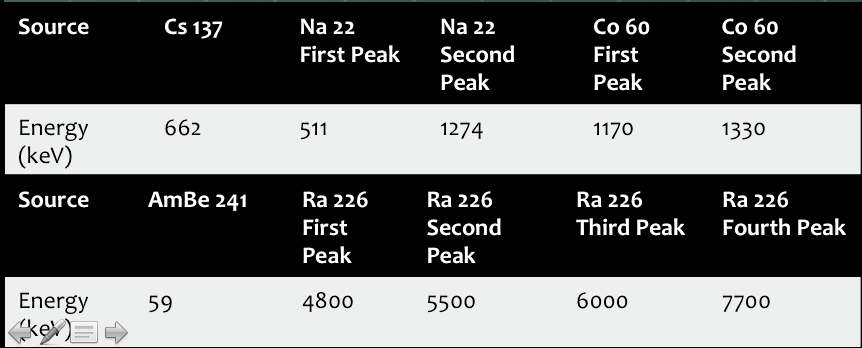
\includegraphics[width=0.5\textwidth]{knownkev.png}
  \caption{Table for each source used and its corresponding keV value}
  \label{fig:workflowedge}
\end{figure} 

In addition to our variables we used several pieces of equipment to collect data. The data compiler, caen, provides a clear user interface and was designed for physics problems of this kind. The power for the PMTs was supplied by a voltage box that could be set to up to 5000 volts. We also used an arduino circuit board and two A2302 temperature probes to collect the temperature in the laboratory while tests were active. Lastly the PMT, crystal, and source was in a light sealed box with cable panels to connect equipment inside and outside. 

\noindent
The above figure is a schematic for the experimental set-up in the laboratory. [Figure 3]. (Place Schematic from PPT)

\begin{figure}
  \centering
    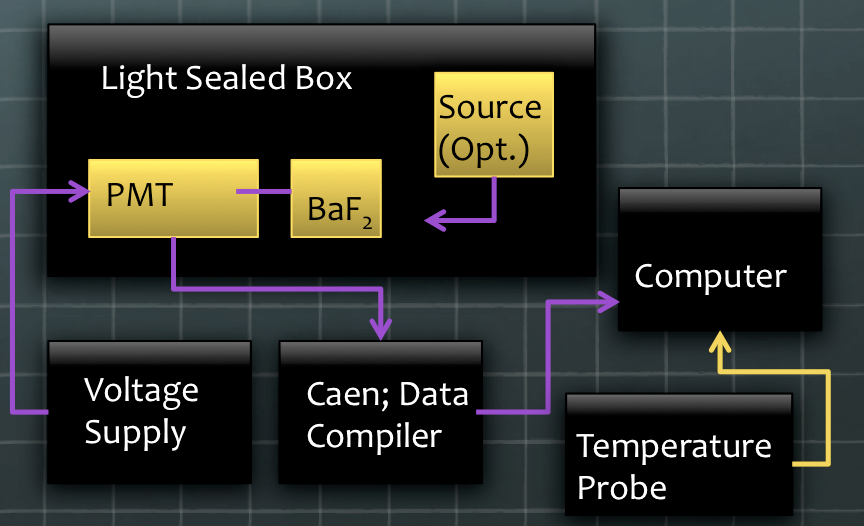
\includegraphics[width=0.5\textwidth]{schem.png}
  \caption{Equipment schematic for experiments}
  \label{fig:workflowedge}
\end{figure} 

\subsection{Experimental Procedure}

In total each source was recorded with each PMT. Before recording any sources, the PMT must be supplied the desired voltage for 12 hours. As the PMT warms up the quantum efficiency is altered and after due time, 12 hours in our case, the PMT's temperature stabilizes. The arduino probe's temperature record must also be launched to ensure the PMT is not affected from external heat fluctuations. 

For a given PMT the voltage and settings on the caen data compiler must remain the same for each source. Depending on the quantum efficiency of the PMT the voltage should be set to maximize the gain and minimize background noise;  the higher the voltage, the higher the gain. The threshold, bin size, and gate length must also be set. Raising the threshold diminishes background noise, but can also dimish noise from the source. The bin size sets a relative scale for the energy counts and must take into account the dispersion of source peaks so the highest source is not above the recorded channel. The gate length is in ns and regulates the amount of light detected for each collection point; it can also be used to lower the portion of the slow component seen. 

\subsubsection{Evaluating a PMT}

To begin collection with a PMT the lense and crystal must both be cleaned. The crystal is then wrapped on 5 of the faces with a shielding material to prevent light from leaving out the sides and not into the PMT. The open face of the crystal is secured onto the PMT with grease to optimize light collected. Then the PMT and crystal are placed in the light sealed box and connected with coaxial cables to the voltage supply and caen. After the PMT has been left on for at least 12 hours the sources can be evaluated. Following standard radiation safety procedure then place a source in the light sealed box within a couple inches of the crystal to increase interactions. Ensure the parameters are adequately set, laboratory temparature is being recorded, and data points are being collected. Once the caen has enough counts in each bin to show an energy peak in the histogram at the desired resolution, data should be saved, and the process repeated with the three other sources and then the crystal alone with the PMT for Ra 226. 

Each source varies in rate of decay and each PMT varies in the amount of light it can record. Tests varied widely in length required to record enough data points for the histogram [Figure 4]. 

\begin{figure}
  \centering
    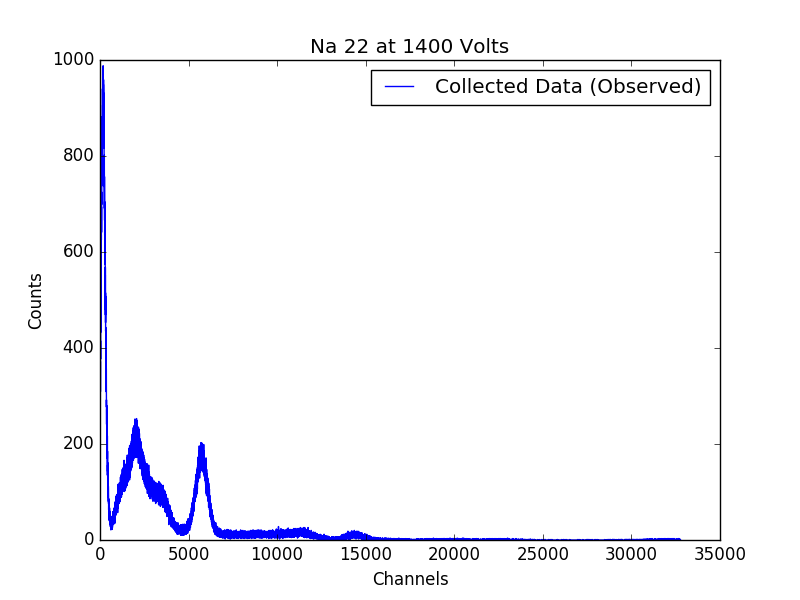
\includegraphics[width=0.5\textwidth]{na.png}
  \caption{Na 22 Solarblind PMT total energy histogram}
  \label{fig:workflowedge}
\end{figure} 


\subsection{Data Analysis}

Before begining data collection we created unique python scripts to analyze our anticpated data. The first program extracts the histogram for each source from a txt file and fits the energy peaks with a Gaussian. The gaussian fit produces the central peak value in channels for each energy level. Then the known decay values for each source are used to find the conversion from channels to keV. The conversion for each Ra 226 peak produces the expected keV value from channels. This is then compared to the known Ra 226 decays in keV to find the quenching factor, $\alpha_Q$ at each energy. We repeated this process for each PMT and recorded the quenching factors. 

The second program is also repeated for each PMT. The script convolves the QE specifications from each PMT manufacturer and the emission spectrum for Barium Fluoride which produces a four gaussian representation of the fast and slow component proportions. The proportion of area from each component produces $E_s$ and $E_f$. 

Lastly a final script requires the input of the quenching factor and component proportions as global lists. The subsequent functions then produces four energy plots of $\alpha_Q = E_f * \alpha_f + E_s * \alpha_s$ where $\alpha_Q$ using data from each PMT. The closest intersection of the line represents ($\alpha_s, \alpha_f$), the final quenching factors. To find these points we created a mathematica script and solved the minimized the cost function analytically. From this process the covariance matrix can be formed to determine the errors on each value. The four ($\alpha_s, \alpha_f$) and their respective ($\sigma_s, \sigma_f$) are then imported back to the python script to plot each fast and slow value against the corresponding energies for the final quenching factors as a function of energy in MeV. 


\section{Results}

We found $\alpha_Q, E_f,$ and $E_s$ for each PMT. $\alpha_f$ and $\alpha_s$ were determined at the four Ra 226 energy peak values, 4.8, 5.5, 6.0, and 7.7 MeV. The fast and slow proportion was also found for each PMT. For each PMT we fit every source with a Gaussian Fits [Figures 5 and 6] which yielding the following parameter fits [Figure 7]. 

\begin{figure}[H]
  \centering
  \begin{minipage}[b]{0.4\textwidth}
    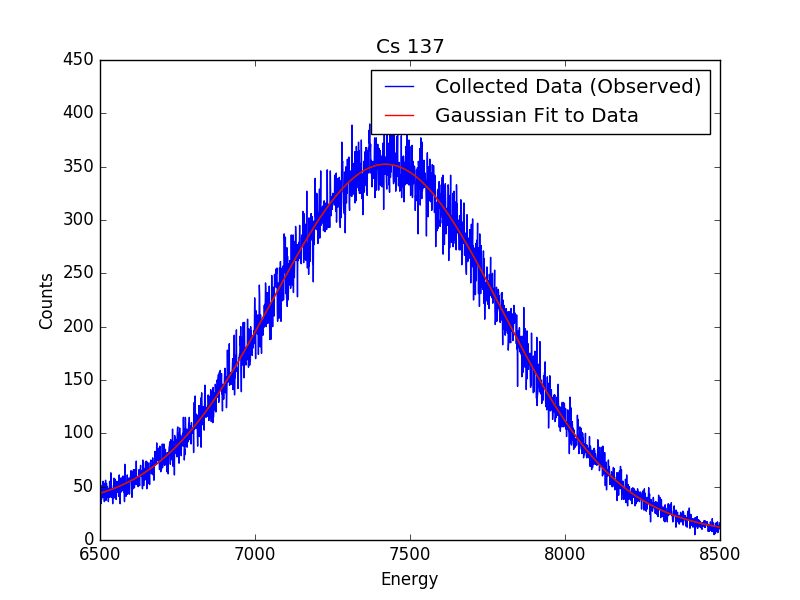
\includegraphics[width=\textwidth]{Cs137.png}
    \caption{An Example of a Gaussian Fit, UV PMT}
  \end{minipage}
  \hfill
  \begin{minipage}[b]{0.4\textwidth}
    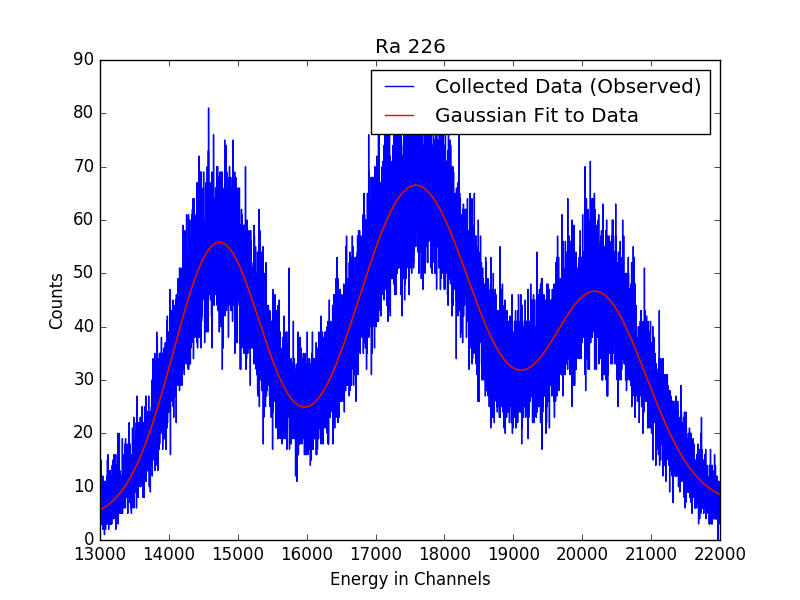
\includegraphics[width=\textwidth]{Ra1.png}
    \caption{An Example of a Gaussian Fit, UV PMT}
  \end{minipage}
\end{figure}

\begin{figure}
  \centering
    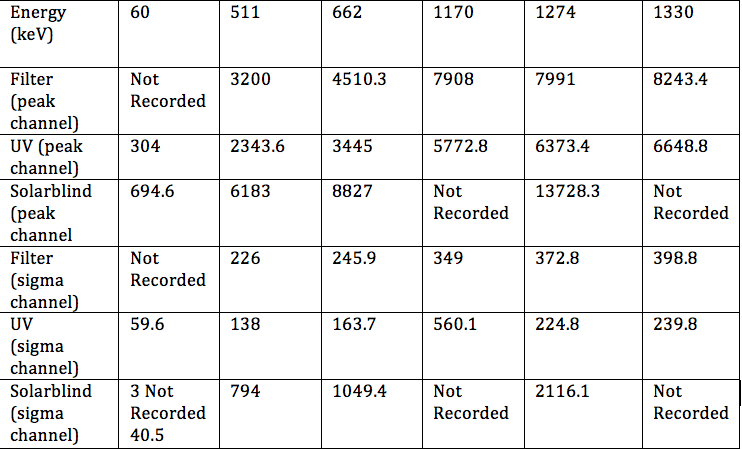
\includegraphics[width=0.5\textwidth]{gaussfits.png}
  \caption{Table with the recorded gaussian fit parameters}
  \label{fig:workflowedge}
\end{figure} 

\noindent
Using the peak value and sigma the keV to channels conversion [Figures 8 to 10] was determined for each PMT; UV with shortpass filter, UV, Solarblind = [6.33012509, 4.984, 12.0694256] 

\begin{figure}[H]
  \centering
  \begin{minipage}[b]{0.4\textwidth}
    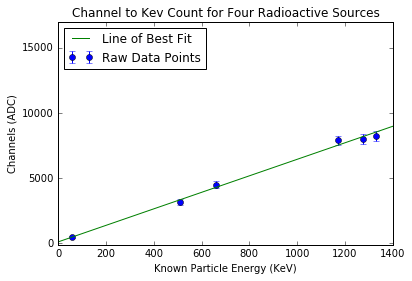
\includegraphics[width=\textwidth]{chanf.png}
    \caption{UV with filter Calibration Function}
  \end{minipage}
  \hfill
  \begin{minipage}[b]{0.4\textwidth}
    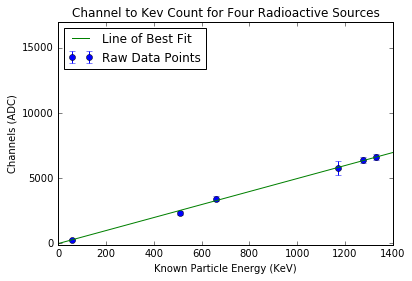
\includegraphics[width=\textwidth]{chanuv.png}
    \caption{UV Calibration Function}
  \end{minipage}
\end{figure}

\begin{figure}
  \centering
    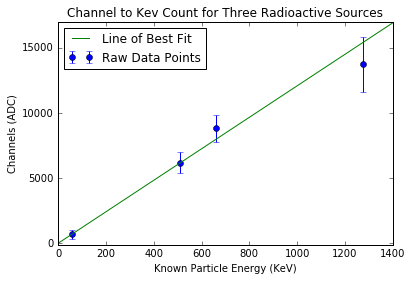
\includegraphics[width=0.5\textwidth]{chansb.png}
  \caption{Solarblind Calibration Function}
  \label{fig:workflowedge}
\end{figure} 


The inverse slope of the best fit line multiplied by the Ra 226 peak channel values yielded the expected keV values, which then determined the quenching factors $\alpha_Q$ [Figures 11 to 13]. 

\setlength{\parskip}{2em}
\noindent
Quenching Factor UV with filter = [2.9762807168446512, 2.8493222446691253, 2.7046015279015254, 2.459904200468519]
\noindent
Quenching Factor UV = [3.269623267619078, 3.1364744649952887, 2.9771822748456365, 2.702319438114875]
\noindent
Quenching Factor Solarblind = [5.155991131280197, 4.789453699584773, 4.475792970019146, 4.166273337999092]

\begin{figure}[H]
  \centering
  \begin{minipage}[b]{0.4\textwidth}
    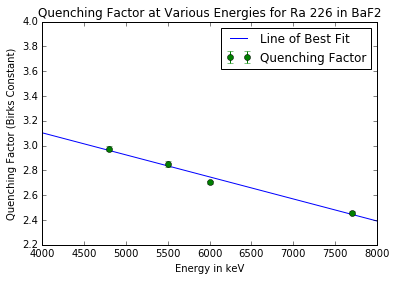
\includegraphics[width=\textwidth]{qff.png}
    \caption{UV with filter Quenching Factors}
  \end{minipage}
  \hfill
  \begin{minipage}[b]{0.4\textwidth}
    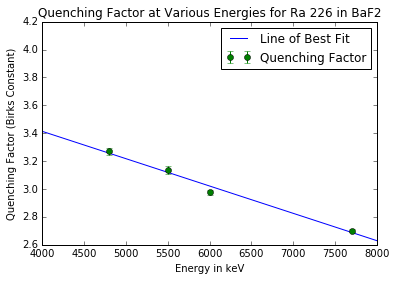
\includegraphics[width=\textwidth]{qfuv.png}
    \caption{UV Quenching Factors}
  \end{minipage}
\end{figure}
 
\begin{figure}[H]
  \centering
  \begin{minipage}[b]{0.4\textwidth}
    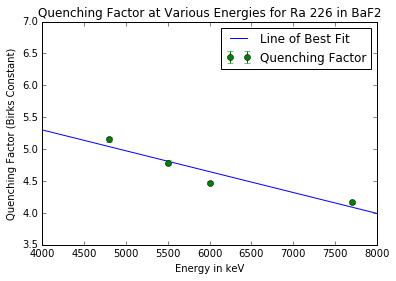
\includegraphics[width=\textwidth]{qfsb.png}
    \caption{Solarblind Quenching Factors}
  \end{minipage}
  \hfill
  \begin{minipage}[b]{0.4\textwidth}
    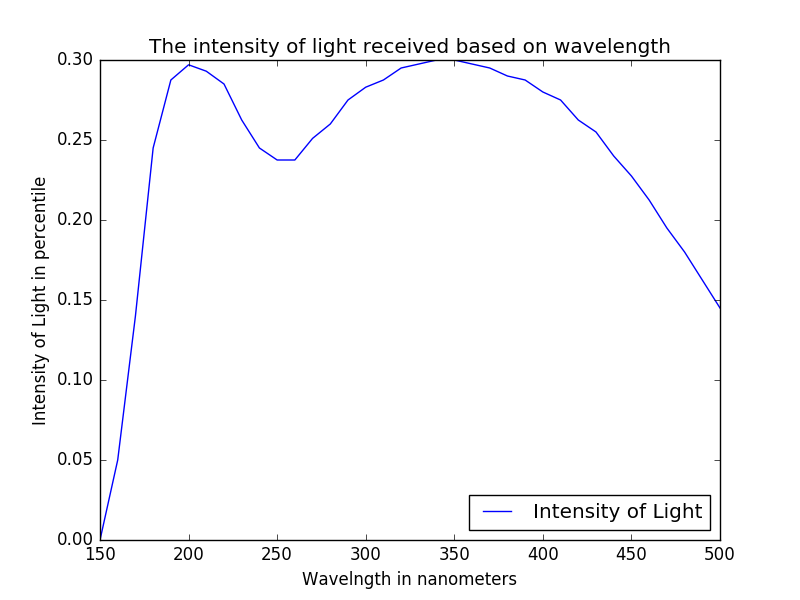
\includegraphics[width=\textwidth]{PMT1QE.png}
    \caption{UV Quenching Factors}
  \end{minipage}
\end{figure}


The emmission spectrum of Barium Flouride was plotted and fitted with four gaussians. Using this fit we convolved each QE spectrum [Figure 14] to find $E_f$ and $E_s$ [Figures 15 to 17]. 

\setlength{\parskip}{2em}
\noindent
Fast and Slow Proportions UV with filter = (0.10416262087647044, 0.8958373791235295)
\noindent
Fast and Slow Proportions UV = (0.11286243062670365, 0.8871375693732964)
\noindent
Fast and Slow Proportions Solarblind = (0.5585223540278348, 0.4414776459721652)

\begin{figure}[H]
  \centering
  \begin{minipage}[b]{0.4\textwidth}
    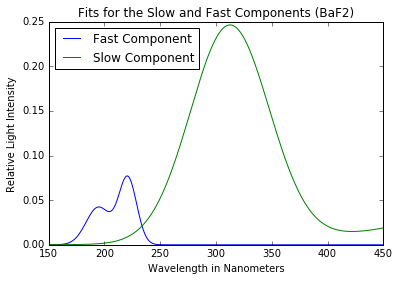
\includegraphics[width=\textwidth]{convf.png}
    \caption{UV with filter Convolution}
  \end{minipage}
  \hfill
  \begin{minipage}[b]{0.4\textwidth}
    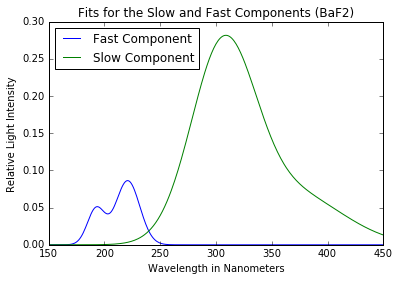
\includegraphics[width=\textwidth]{convuv.png}
    \caption{UV Convolution}
  \end{minipage}
\end{figure}

\begin{figure}
  \centering
    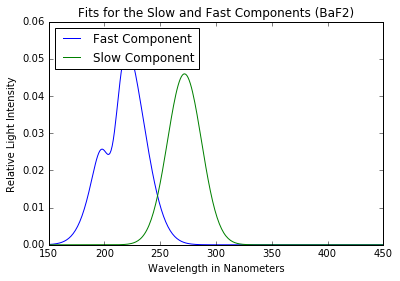
\includegraphics[width=0.5\textwidth]{convsb.png}
  \caption{Solarblind Convolution}
  \label{fig:workflowedge}
\end{figure}

\noindent
We plotted our determined values in this form at each energy $\alpha_Q = E_f * \alpha_f + E_s * \alpha_s$ [Figures 18 to 21]. Solving for the best ($\alpha_s, \alpha_f$) at each energy level the quneching factor as a function of energy was found to be $\alpha_s = -0.1398072 * Energy + 4.13497323$ and $\alpha_f = -0.45007859 * Energy + 11.23363402$ with errors of $\sigma_s = [1.36287, 1.31089, 1.2333, 1.10977]$ and $\sigma_f = [0.0290772, 0.0310162, 0.0319127, 0.0313639]$ [Figure 22]. These functions can be used in future high energy physic experiments to isolate the fast component in $BaF_2$. Beyond experimental analysis on the quenching factor, the physical phenomenom that determine the constant will be explored. 

\begin{figure}[H]
  \centering
  \begin{minipage}[b]{0.4\textwidth}
    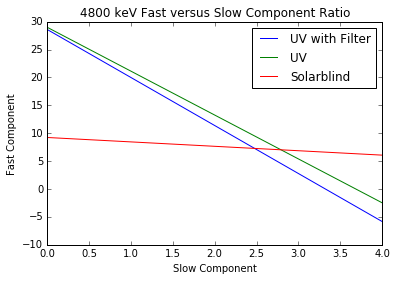
\includegraphics[width=\textwidth]{first.png}
    \caption{4800 Slow versus Fast Componets}
  \end{minipage}
  \hfill
  \begin{minipage}[b]{0.4\textwidth}
    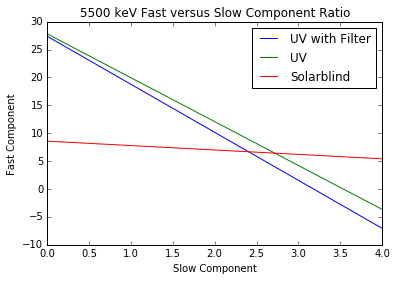
\includegraphics[width=\textwidth]{second.png}
    \caption{5500 Slow versus Fast Componets}
  \end{minipage}
\end{figure}

\begin{figure}[H]
  \centering
  \begin{minipage}[b]{0.4\textwidth}
    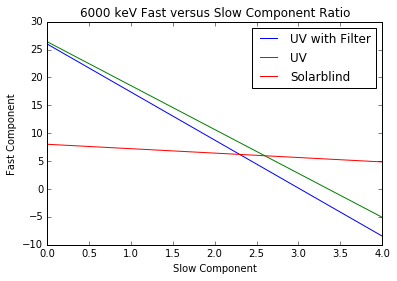
\includegraphics[width=\textwidth]{third.png}
    \caption{6000 Slow versus Fast Componets}
  \end{minipage}
  \hfill
  \begin{minipage}[b]{0.4\textwidth}
    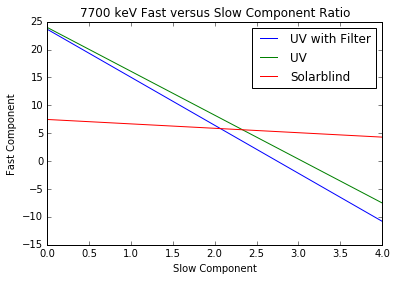
\includegraphics[width=\textwidth]{fourth.png}
    \caption{7700 Slow versus Fast Componets}
  \end{minipage}
\end{figure}

\begin{figure}
  \centering
    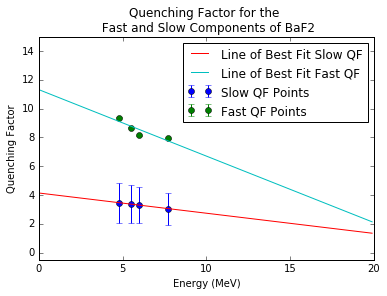
\includegraphics[width=0.5\textwidth]{qf.png}
  \caption{Final Quenching Factor Function}
  \label{fig:workflowedge}
\end{figure} 


\section{Acknowledgements}

The measurement of the quenching factor for barium fluoride crystals was made possible by the California Institue of Technology and its Student Faculty Programs office for the Summer Undergraduate Research Fellowship. The involvement and support of Professor David Hitlin, Jake Kim, and Jason Trevor and the High Energy Physics group was crucial to the completion and implementation of this research. 




\end{document} 

































